\tikzstyle{block}=[node distance=5.2em, text width=4.5em, minimum height=7em, align=center, rounded corners=8pt, font=\small]
\tikzstyle{my brace}=[decorate, decoration={brace, amplitude=10pt}]
\tikzstyle{horz}=[node distance=2.7em]
\tikzstyle{vert}=[node distance=4em]
\begin{figure}[b]
	\centering
	\begin{tikzpicture}[scale=0.95, every node/.style={transform shape}]
		% Draw the blocks
		\node[block, fill=blue!30](dc){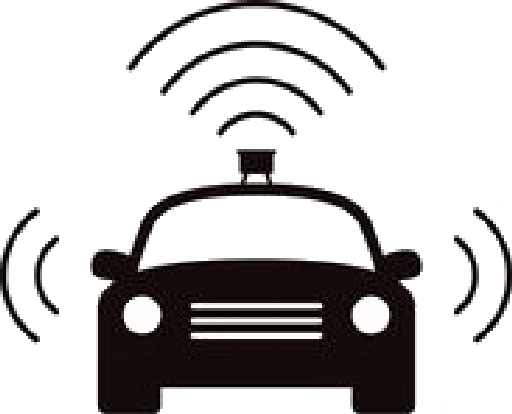
\includegraphics[width=4em]{data_collection.png} \\ Data collection};
		\node[block, fill=blue!30, right of=dc](dp){
\includegraphics[width=2.5em]{data_processing.png} \\ Data preprocessing};
		\node[block, fill=green!30, right of=dp](ed){
\includegraphics[width=4.2em]{event_detection.png} \\ Activity detection};
		\node[block, fill=green!30, right of=ed](s){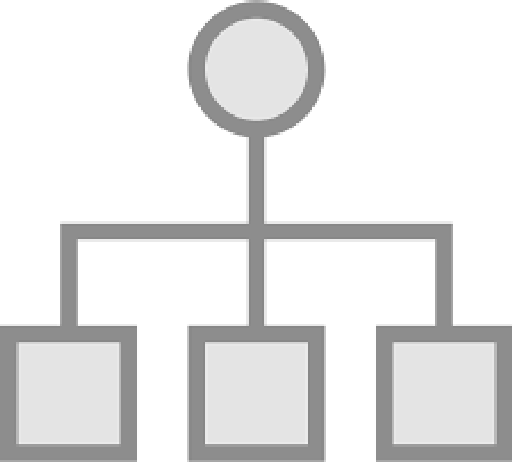
\includegraphics[width=3em]{scenario_mining.png} \\ Scenario mining};
		\node[block, fill=green!30, right of=s](p){
\includegraphics[width=3em]{parametrisation.png} \\ Parame-trization};
		\node[block, fill=green!30, right of=p](tc){
\includegraphics[width=3.2em]{scenarios.png} \\ Test case genera-tion};
		\node[block, fill=red!30, right of=tc](sim){
\includegraphics[width=4em]{simulation.png} \\ Simulation};
		\node[block, fill=red!30, right of=sim](eval){
\includegraphics[width=3em]{evaluation.png} \\ Evaluation};
		
		% Show completeness part
		\node[horz, left of=ed](b1){};
		\node[vert, below of=b1](b2){};
		\node[horz, right of=tc](b3){};
		\node[vert, below of=b3](b4){};
		\draw[my brace](b4) -- (b2) node[midway, yshift=-2em, align=center]{Completeness};
	\end{tikzpicture}
	\vspace{-1em}
	\caption{Schematic overview of the process of the assessment of an automated vehicle using real-world data. The green blocks are the focus of the PhD research.}
	\label{fig:scheme}
\end{figure}
